\chapter{Component separation: finding the cells}\label{ch:separation}

\section{The problem}

A blood specimen is a mixture. At site $i$ its methylation is, to good approximation,
\begin{equation}
  \beta_i=\sum_g f_g\,\mu_{g,i}+\epsilon_i,\qquad f_g\ge0,\ \ \sum_g f_g=1,
  \label{eq:mix}
\end{equation}
where $\mu_{g,i}$ is the healthy methylation of cell group $g$ at site $i$ and $f_g$ its fraction of the DNA in the tube. This is the
methylome's component separation, and it is solved by constrained least squares on a set of sites that separate the cells
(markers)~\cite{Houseman2012,Salas2022}. On the sky the same equation has frequencies in place of sites and emission laws in place
of cell profiles.

\section{Two jobs, kept apart}

The fraction of a cell in the specimen does not decide whether the cell is healthy; it decides how much change a reading could detect. In chain v3 the composition
step (Stage~A) does two things and nothing else:
\begin{enumerate}
\item it supplies the neutrophil fraction, which decides whether a reading is made and how large a change it could show;
\item it supplies the fractions from which the specimen's own healthy expectation is built (Eq.~\eqref{eq:metawb}).
\end{enumerate}
It never supplies a cell's $A$. The neutrophil is read on its own identity sites (Chapter~\ref{ch:identity}).

\section{The solver}

Stage~A solves eight groups: neutrophils, eosinophils, basophils, monocytes, B cells, NK cells, CD4 T cells and CD8 T cells, from purified
EPIC arrays of healthy donors~\cite{Salas2018,Salas2022} processed by the chain's own Stage~1.
The markers are sites chosen by a stated rule: not a neutrophil identity site; steady within the group; a clear margin
against every other group's mean; a capped number per group. Composition is non-negative least squares on those markers, normalised to sum one.
Enough of the markers must be measured, or the composition is not solved and no reading is made. The mean absolute residual
of the fit is recorded with every specimen. \calibrated{} (profiles and markers)

Figure~\ref{fig:p4_markers} shows the eight templates at the markers.

\begin{figure}[htbp]\centering
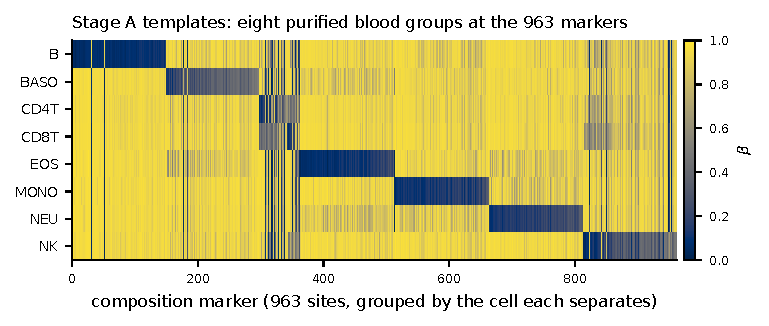
\includegraphics[width=0.98\textwidth]{figures/part6/fig_p4_13_markers.pdf}
\caption{Stage~A templates: healthy $\beta$ of eight purified EPIC blood groups~\cite{Salas2018,Salas2022} at the composition markers, grouped by
the group each marker separates most. T-cell markers are fewest, because few sites separate the two T-cell groups
from each other and from NK cells by the margin. \calibrated}
\label{fig:p4_markers}
\end{figure}

The solver runs on the same platform, through the same calibration, and on the same reference cells as the expectation it feeds.


\section{Fraction and the reading}

A neutrophil that is a small share of the DNA moves the whole-blood reading less. The chain does not use a fixed share as a gate. It reads
neutrophils when they are above a read line and enough of the identity sites are measured; below the line the fraction is printed and $A$ is withheld. Above the line every tared reading carries its own detection
limit (Chapter~\ref{ch:instrument}). A cell that is a smaller share of the specimen moves the reading less, while the healthy spread does not
grow, so the per-specimen detection limit, not a fixed share, is the right statement. \derived

\paragraph{Why an absent cell is not read.} A cell that is not in the specimen still has identity sites, and the array still reports
a $\beta$ at each of them. Those values belong to the cells that are present. Where the present cells hold a site differently from
the absent cell, their mixture moves toward a coin flip, and the absent cell's reading moves toward the far end of its gauge.
\derived{} On 318 healthy whole-blood arrays from four laboratories, the identity sites of cell groups absent from blood read at or
near the largest value their gauge allows, one of them at 100~\% of it. \measured{} A reading near the far end on a cell below its read line is an artefact of absence, not a severity. That
is why the chain reads a cell only above its read line, and below it prints the fraction and never a corrected $A$.

\paragraph{What fraction still does to the reading.} In a second laboratory, tared whole-blood Met-A rose with neutrophil fraction by about $+0.12$
per unit fraction ($\rho\approx0.31$), after the composition-matched expectation and a median tare. \measured{} The expectation
profiles come from one laboratory and do not cancel fully in another. In a development fit with $f_{\rm neu}$ and $N$, made after looking at these data, the dependence fell to
$\rho=-0.02$. \fitted{} Chain v3 uses no fitted correction: it measures $N$ and withholds the gauge state when $N$
lies outside the purified reference arrays' range (Chapter~\ref{ch:chain}).

\section{The transfer function}

A composition solver explains away anything that looks like a change in composition. A real change in a cell's methylation at sites shared with
another cell is partly absorbed as a change in fractions, and the signal shrinks. In CMB language this is the pipeline's transfer function: the
analysis filters the signal it is meant to find. Chain v3 limits it by construction: no Stage~A marker is a neutrophil identity site. The
construction was tested. On six known mixtures with a simulated 2~\% loss of the neutrophil pattern, the tared reading rose above 1.05 on 6 of 6;
when the fraction was instead re-fitted on the neutrophil sites, the fit absorbed the loss and 0 of 6 rose above 1.05. \measured{} The transfer of a real change through the solver, measured by injecting known damage into
real mixtures, is not yet built. \openprob

\section{A second opinion}

Cosmology never trusted one separation method. A second, independent solver whose composition is shown beside the primary's as a cross-check is
not yet built in chain v3. \openprob

When a second solver disagrees with the first on every specimen, the disagreement is information about the reference: it marks the
cells the reference cannot separate on the sites in use. The response is to measure that separability, not to switch the second
solver off. \interp

\section{Cells the solver does not hold}

Stage~A holds eight blood groups and nothing else. A cell outside them, an epithelial cell in blood or a blast in leukaemic blood, has no template
and its DNA is spread over the eight. The chain does not detect such a cell; the recorded residual of the fit is the only sign of it. One record
shows why this matters. In leukaemic blood dominated by blasts, the neutrophil-led reading stayed near 1, and reading a blast against the neutrophil
floor is not what the gauge defines. \measured{} A joint fit in which non-blood templates compete for
mass with blood, and a dominant-cell call that names the cell to be read, are not yet built. \openprob

\section{Finding a trace cell}\label{sec:p4tracecell}

A non-negative least-squares fit sets a component to exactly zero whenever adding it does not lower the residual; that is the
optimality condition of the constrained fit. \derived{} A cell whose contribution is smaller than the array noise on the markers
therefore returns a fraction of zero more often than its true value. On 450K arrays from four laboratories, a template fit of this
kind detected four solid-tissue cell types spiked into real whole-blood arrays only from 2--5~\% of the DNA. \measured

\begin{keybox}[title=Status]
Chain v3 holds no non-blood template and detects no trace cell. A detection line that respects the rule of Chapter~\ref{ch:translation}
has to come from references run beside the specimen or from the instrument's own noise, not from a stored panel of people. \openprob
\end{keybox}
